%%
% Copyright (c) 2017 - 2024, Pascal Wagler;
% Copyright (c) 2014 - 2024, John MacFarlane
%
% All rights reserved.
%
% Redistribution and use in source and binary forms, with or without
% modification, are permitted provided that the following conditions
% are met:
%
% - Redistributions of source code must retain the above copyright
% notice, this list of conditions and the following disclaimer.
%
% - Redistributions in binary form must reproduce the above copyright
% notice, this list of conditions and the following disclaimer in the
% documentation and/or other materials provided with the distribution.
%
% - Neither the name of John MacFarlane nor the names of other
% contributors may be used to endorse or promote products derived
% from this software without specific prior written permission.
%
% THIS SOFTWARE IS PROVIDED BY THE COPYRIGHT HOLDERS AND CONTRIBUTORS
% "AS IS" AND ANY EXPRESS OR IMPLIED WARRANTIES, INCLUDING, BUT NOT
% LIMITED TO, THE IMPLIED WARRANTIES OF MERCHANTABILITY AND FITNESS
% FOR A PARTICULAR PURPOSE ARE DISCLAIMED. IN NO EVENT SHALL THE
% COPYRIGHT OWNER OR CONTRIBUTORS BE LIABLE FOR ANY DIRECT, INDIRECT,
% INCIDENTAL, SPECIAL, EXEMPLARY, OR CONSEQUENTIAL DAMAGES (INCLUDING,
% BUT NOT LIMITED TO, PROCUREMENT OF SUBSTITUTE GOODS OR SERVICES;
% LOSS OF USE, DATA, OR PROFITS; OR BUSINESS INTERRUPTION) HOWEVER
% CAUSED AND ON ANY THEORY OF LIABILITY, WHETHER IN CONTRACT, STRICT
% LIABILITY, OR TORT (INCLUDING NEGLIGENCE OR OTHERWISE) ARISING IN
% ANY WAY OUT OF THE USE OF THIS SOFTWARE, EVEN IF ADVISED OF THE
% POSSIBILITY OF SUCH DAMAGE.
%%

%%
% This is the Eisvogel pandoc LaTeX template.
%
% For usage information and examples visit the official GitHub page:
% https://github.com/Wandmalfarbe/pandoc-latex-template
%%

% Options for packages loaded elsewhere
\PassOptionsToPackage{unicode}{hyperref}
\PassOptionsToPackage{hyphens}{url}
\PassOptionsToPackage{dvipsnames,svgnames,x11names,table}{xcolor}
%
\documentclass[
  paper=a4,
  ,captions=tableheading
]{scrartcl}
\usepackage{amsmath,amssymb}
% Use setspace anyway because we change the default line spacing.
% The spacing is changed early to affect the titlepage and the TOC.
\usepackage{setspace}
\setstretch{1.2}
\usepackage{iftex}
\ifPDFTeX
  \usepackage[T1]{fontenc}
  \usepackage[utf8]{inputenc}
  \usepackage{textcomp} % provide euro and other symbols
\else % if luatex or xetex
  \usepackage{unicode-math} % this also loads fontspec
  \defaultfontfeatures{Scale=MatchLowercase}
  \defaultfontfeatures[\rmfamily]{Ligatures=TeX,Scale=1}
\fi
\usepackage{lmodern}
\ifPDFTeX\else
  % xetex/luatex font selection
\fi
% Use upquote if available, for straight quotes in verbatim environments
\IfFileExists{upquote.sty}{\usepackage{upquote}}{}
\IfFileExists{microtype.sty}{% use microtype if available
  \usepackage[]{microtype}
  \UseMicrotypeSet[protrusion]{basicmath} % disable protrusion for tt fonts
}{}
\makeatletter
\@ifundefined{KOMAClassName}{% if non-KOMA class
  \IfFileExists{parskip.sty}{%
    \usepackage{parskip}
  }{% else
    \setlength{\parindent}{0pt}
    \setlength{\parskip}{6pt plus 2pt minus 1pt}}
}{% if KOMA class
  \KOMAoptions{parskip=half}}
\makeatother
\usepackage{xcolor}
\definecolor{default-linkcolor}{HTML}{A50000}
\definecolor{default-filecolor}{HTML}{A50000}
\definecolor{default-citecolor}{HTML}{4077C0}
\definecolor{default-urlcolor}{HTML}{4077C0}
\usepackage[top=1in,bottom=1in]{geometry}
\usepackage{longtable,booktabs,array}
\usepackage{calc} % for calculating minipage widths
% Correct order of tables after \paragraph or \subparagraph
\usepackage{etoolbox}
\makeatletter
\patchcmd\longtable{\par}{\if@noskipsec\mbox{}\fi\par}{}{}
\makeatother
% Allow footnotes in longtable head/foot
\IfFileExists{footnotehyper.sty}{\usepackage{footnotehyper}}{\usepackage{footnote}}
\makesavenoteenv{longtable}
% add backlinks to footnote references, cf. https://tex.stackexchange.com/questions/302266/make-footnote-clickable-both-ways
\usepackage{footnotebackref}
\usepackage{graphicx}
\makeatletter
\newsavebox\pandoc@box
\newcommand*\pandocbounded[1]{% scales image to fit in text height/width
  \sbox\pandoc@box{#1}%
  \Gscale@div\@tempa{\textheight}{\dimexpr\ht\pandoc@box+\dp\pandoc@box\relax}%
  \Gscale@div\@tempb{\linewidth}{\wd\pandoc@box}%
  \ifdim\@tempb\p@<\@tempa\p@\let\@tempa\@tempb\fi% select the smaller of both
  \ifdim\@tempa\p@<\p@\scalebox{\@tempa}{\usebox\pandoc@box}%
  \else\usebox{\pandoc@box}%
  \fi%
}
% Set default figure placement to htbp
% Make use of float-package and set default placement for figures to H.
% The option H means 'PUT IT HERE' (as  opposed to the standard h option which means 'You may put it here if you like').
\usepackage{float}
\floatplacement{figure}{H}
\makeatother
\setlength{\emergencystretch}{3em} % prevent overfull lines
\providecommand{\tightlist}{%
  \setlength{\itemsep}{0pt}\setlength{\parskip}{0pt}}
\setcounter{secnumdepth}{-\maxdimen} % remove section numbering
\ifLuaTeX
\usepackage[bidi=basic]{babel}
\else
\usepackage[bidi=default]{babel}
\fi
\babelprovide[main,import]{english}
% get rid of language-specific shorthands (see #6817):
\let\LanguageShortHands\languageshorthands
\def\languageshorthands#1{}
\makeatletter
\@ifpackageloaded{subfig}{}{\usepackage{subfig}}
\@ifpackageloaded{caption}{}{\usepackage{caption}}
\captionsetup[subfloat]{margin=0.5em}
\AtBeginDocument{%
\renewcommand*\figurename{Figura}
\renewcommand*\tablename{Tabla}
}
\AtBeginDocument{%
\renewcommand*\listfigurename{Lista de Figuras}
\renewcommand*\listtablename{Lista de Tablas}
}
\newcounter{pandoccrossref@subfigures@footnote@counter}
\newenvironment{pandoccrossrefsubfigures}{%
\setcounter{pandoccrossref@subfigures@footnote@counter}{0}
\begin{figure}\centering%
\gdef\global@pandoccrossref@subfigures@footnotes{}%
\DeclareRobustCommand{\footnote}[1]{\footnotemark%
\stepcounter{pandoccrossref@subfigures@footnote@counter}%
\ifx\global@pandoccrossref@subfigures@footnotes\empty%
\gdef\global@pandoccrossref@subfigures@footnotes{{##1}}%
\else%
\g@addto@macro\global@pandoccrossref@subfigures@footnotes{, {##1}}%
\fi}}%
{\end{figure}%
\addtocounter{footnote}{-\value{pandoccrossref@subfigures@footnote@counter}}
\@for\f:=\global@pandoccrossref@subfigures@footnotes\do{\stepcounter{footnote}\footnotetext{\f}}%
\gdef\global@pandoccrossref@subfigures@footnotes{}}
\@ifpackageloaded{float}{}{\usepackage{float}}
\floatstyle{ruled}
\@ifundefined{c@chapter}{\newfloat{codelisting}{h}{lop}}{\newfloat{codelisting}{h}{lop}[chapter]}
\floatname{codelisting}{Listing}
\newcommand*\listoflistings{\listof{codelisting}{Listas del Documento}}
\makeatother
\usepackage{bookmark}
\IfFileExists{xurl.sty}{\usepackage{xurl}}{} % add URL line breaks if available
\urlstyle{same}
\hypersetup{
  pdftitle={Gestión de Requerimientos JEP},
  pdfauthor={Versión actual: 1.12af1e5 - Compilación para entrega - Fri, 8 Nov 2024 16:06:05 +0000},
  pdflang={en},
  pdfsubject={Implementación Proyecto JEP},
  pdfkeywords={Integración, Interoperabilidad, JEP, Softgic, Caso de
uso},
  hidelinks,
  breaklinks=true,
  pdfcreator={LaTeX via pandoc with the Eisvogel template}}
\title{Gestión de Requerimientos JEP}
\usepackage{etoolbox}
\makeatletter
\providecommand{\subtitle}[1]{% add subtitle to \maketitle
  \apptocmd{\@title}{\par {\large #1 \par}}{}{}
}
\makeatother
\subtitle{Implementación Proyecto Evolución de Interoperabilidad JEP,
Softgic}
\author{Versión actual: 1.12af1e5 - Compilación para entrega - Fri, 8
Nov 2024 16:06:05 +0000}
\date{2024-11-8}



%%
%% added
%%


%
% for the background color of the title page
%
\usepackage{pagecolor}
\usepackage{afterpage}

%
% break urls
%
\PassOptionsToPackage{hyphens}{url}

%
% When using babel or polyglossia with biblatex, loading csquotes is recommended
% to ensure that quoted texts are typeset according to the rules of your main language.
%
\usepackage{csquotes}

%
% captions
%
\definecolor{caption-color}{HTML}{777777}
\usepackage[font={stretch=1.2}, textfont={color=caption-color}, position=top, skip=4mm, labelfont=bf, singlelinecheck=false, justification=raggedright]{caption}
\setcapindent{0em}

%
% blockquote
%
\definecolor{blockquote-border}{RGB}{221,221,221}
\definecolor{blockquote-text}{RGB}{119,119,119}
\usepackage{mdframed}
\newmdenv[rightline=false,bottomline=false,topline=false,linewidth=3pt,linecolor=blockquote-border,skipabove=\parskip]{customblockquote}
\renewenvironment{quote}{\begin{customblockquote}\list{}{\rightmargin=0em\leftmargin=0em}%
\item\relax\color{blockquote-text}\ignorespaces}{\unskip\unskip\endlist\end{customblockquote}}

%
% Source Sans Pro as the default font family
% Source Code Pro for monospace text
%
% 'default' option sets the default
% font family to Source Sans Pro, not \sfdefault.
%
\ifnum 0\ifxetex 1\fi\ifluatex 1\fi=0 % if pdftex
    \usepackage[default]{sourcesanspro}
  \usepackage{sourcecodepro}
  \else % if not pdftex
    \usepackage[default]{sourcesanspro}
  \usepackage{sourcecodepro}

  % XeLaTeX specific adjustments for straight quotes: https://tex.stackexchange.com/a/354887
  % This issue is already fixed (see https://github.com/silkeh/latex-sourcecodepro/pull/5) but the
  % fix is still unreleased.
  % TODO: Remove this workaround when the new version of sourcecodepro is released on CTAN.
  \ifxetex
    \makeatletter
    \defaultfontfeatures[\ttfamily]
      { Numbers   = \sourcecodepro@figurestyle,
        Scale     = \SourceCodePro@scale,
        Extension = .otf }
    \setmonofont
      [ UprightFont    = *-\sourcecodepro@regstyle,
        ItalicFont     = *-\sourcecodepro@regstyle It,
        BoldFont       = *-\sourcecodepro@boldstyle,
        BoldItalicFont = *-\sourcecodepro@boldstyle It ]
      {SourceCodePro}
    \makeatother
  \fi
  \fi

%
% heading color
%
\definecolor{heading-color}{RGB}{40,40,40}
\addtokomafont{section}{\color{heading-color}}
% When using the classes report, scrreprt, book,
% scrbook or memoir, uncomment the following line.
%\addtokomafont{chapter}{\color{heading-color}}

%
% variables for title, author and date
%
\usepackage{titling}
\title{Gestión de Requerimientos JEP}
\author{Versión actual: 1.12af1e5 - Compilación para entrega - Fri, 8
Nov 2024 16:06:05 +0000}
\date{2024-11-8}

%
% tables
%

\definecolor{table-row-color}{HTML}{F5F5F5}
\definecolor{table-rule-color}{HTML}{999999}

%\arrayrulecolor{black!40}
\arrayrulecolor{table-rule-color}     % color of \toprule, \midrule, \bottomrule
\setlength\heavyrulewidth{0.3ex}      % thickness of \toprule, \bottomrule
\renewcommand{\arraystretch}{1.3}     % spacing (padding)


%
% remove paragraph indentation
%
\setlength{\parindent}{0pt}
\setlength{\parskip}{6pt plus 2pt minus 1pt}
\setlength{\emergencystretch}{3em}  % prevent overfull lines

%
%
% Listings
%
%


%
% header and footer
%
\usepackage[headsepline,footsepline]{scrlayer-scrpage}

\newpairofpagestyles{eisvogel-header-footer}{
  \clearpairofpagestyles
  \ihead*{
\includegraphics{include/jeplogo.jpg}}
  \chead*{}
  \ohead*{2024-11-8}
  \ifoot*{Versión actual: 1.12af1e5 - Compilación para entrega - Fri, 8
Nov 2024 16:06:05 +0000}
  \cfoot*{}
  \ofoot*{\thepage}
  \addtokomafont{pageheadfoot}{\upshape}
}
\pagestyle{eisvogel-header-footer}



%%
%% end added
%%

\begin{document}

%%
%% begin titlepage
%%
\begin{titlepage}
\newgeometry{left=6cm}
\newcommand{\colorRule}[3][black]{\textcolor[HTML]{#1}{\rule{#2}{#3}}}
\begin{flushleft}
\noindent
\\[-1em]
\color[HTML]{5F5F5F}
\makebox[0pt][l]{\colorRule[360049]{1.3\textwidth}{4pt}}
\par
\noindent

{
  \setstretch{1.4}
  \vfill
  \noindent {\huge \textbf{\textsf{Gestión de Requerimientos JEP}}}
    \vskip 1em
  {\Large \textsf{Implementación Proyecto Evolución de Interoperabilidad
JEP, Softgic}}
    \vskip 2em
  \noindent {\Large \textsf{Versión actual: 1.12af1e5 - Compilación para
entrega - Fri, 8 Nov 2024 16:06:05 +0000}}
  \vfill
}


\textsf{2024-11-8}
\end{flushleft}
\end{titlepage}
\restoregeometry
\pagenumbering{arabic}

%%
%% end titlepage
%%

% \maketitle


\section{Requerimientos de Integración
JEP}\label{sec:requerimientos-de-integraciuxf3n-jep}

\begin{itemize}
\tightlist
\item
  \hyperref[Introducciuxf3n]{Introducción}
\item
  \hyperref[problema-1-grouping]{Problema 1 (Grouping)}

  \begin{itemize}
  \tightlist
  \item
    \hyperref[levantamiento-constraint]{Levantamiento (Constraint)}
  \item
    \hyperref[contractual-goal]{Contractual (Goal)}
  \item
    \hyperref[reqr3.-integraciuxf3n-con-sistema-conti-x-plani-requirement]{REQR3.
    Integración con Sistema Conti x Plani (Requirement)}
  \item
    \hyperref[soluciuxf3n-1-grouping]{Solución 1 (Grouping)}

    \begin{itemize}
    \tightlist
    \item
      \hyperref[sint1.-integraciuxf3n.-ingreso-a-conti-application-service]{SINT1.
      Integración. Ingreso a Conti (Application Service)}
    \item
      \hyperref[sint2.-integraciuxf3n.-consulta-uxedtem-de-conti-application-service]{SINT2.
      Integración. Consulta ítem de Conti (Application Service)}
    \item
      \hyperref[sint3.-integraciuxf3n.-radicar-uxedtem-application-service]{SINT3.
      Integración. Radicar ítem (Application Service)}
    \item
      \hyperref[sint4.-integraciuxf3n.-generaciuxf3n-de-documentos-application-service]{SINT4.
      Integración. Generación de documentos (Application Service)}
    \end{itemize}
  \item
    \hyperref[comunicaciuxf3n-conti-x-plani-value]{Comunicación Conti x
    Plani (Value)}
  \end{itemize}
\item
  \hyperref[hu.sint1.-integraciuxf3n.-ingreso-a-conti-deliverable]{HU.SINT1.
  Integración. Ingreso a Conti (Deliverable)}
\item
  \hyperref[hu.sint2.-integraciuxf3n.-consulta-uxedtem-de-conti-deliverable]{HU.SINT2.
  Integración. Consulta ítem de Conti (Deliverable)}
\item
  \hyperref[hu.sint3.-integraciuxf3n.-radicar-uxedtem-deliverable]{HU.SINT3.
  Integración. Radicar ítem (Deliverable)}
\item
  \hyperref[hu.sint4.-integraciuxf3n.-generaciuxf3n-de-documentos-deliverable]{HU.SINT4.
  Integración. Generación de documentos (Deliverable)}
\end{itemize}

\subsection{Introducción}\label{sec:introducciuxf3n}

\begin{figure}
\centering
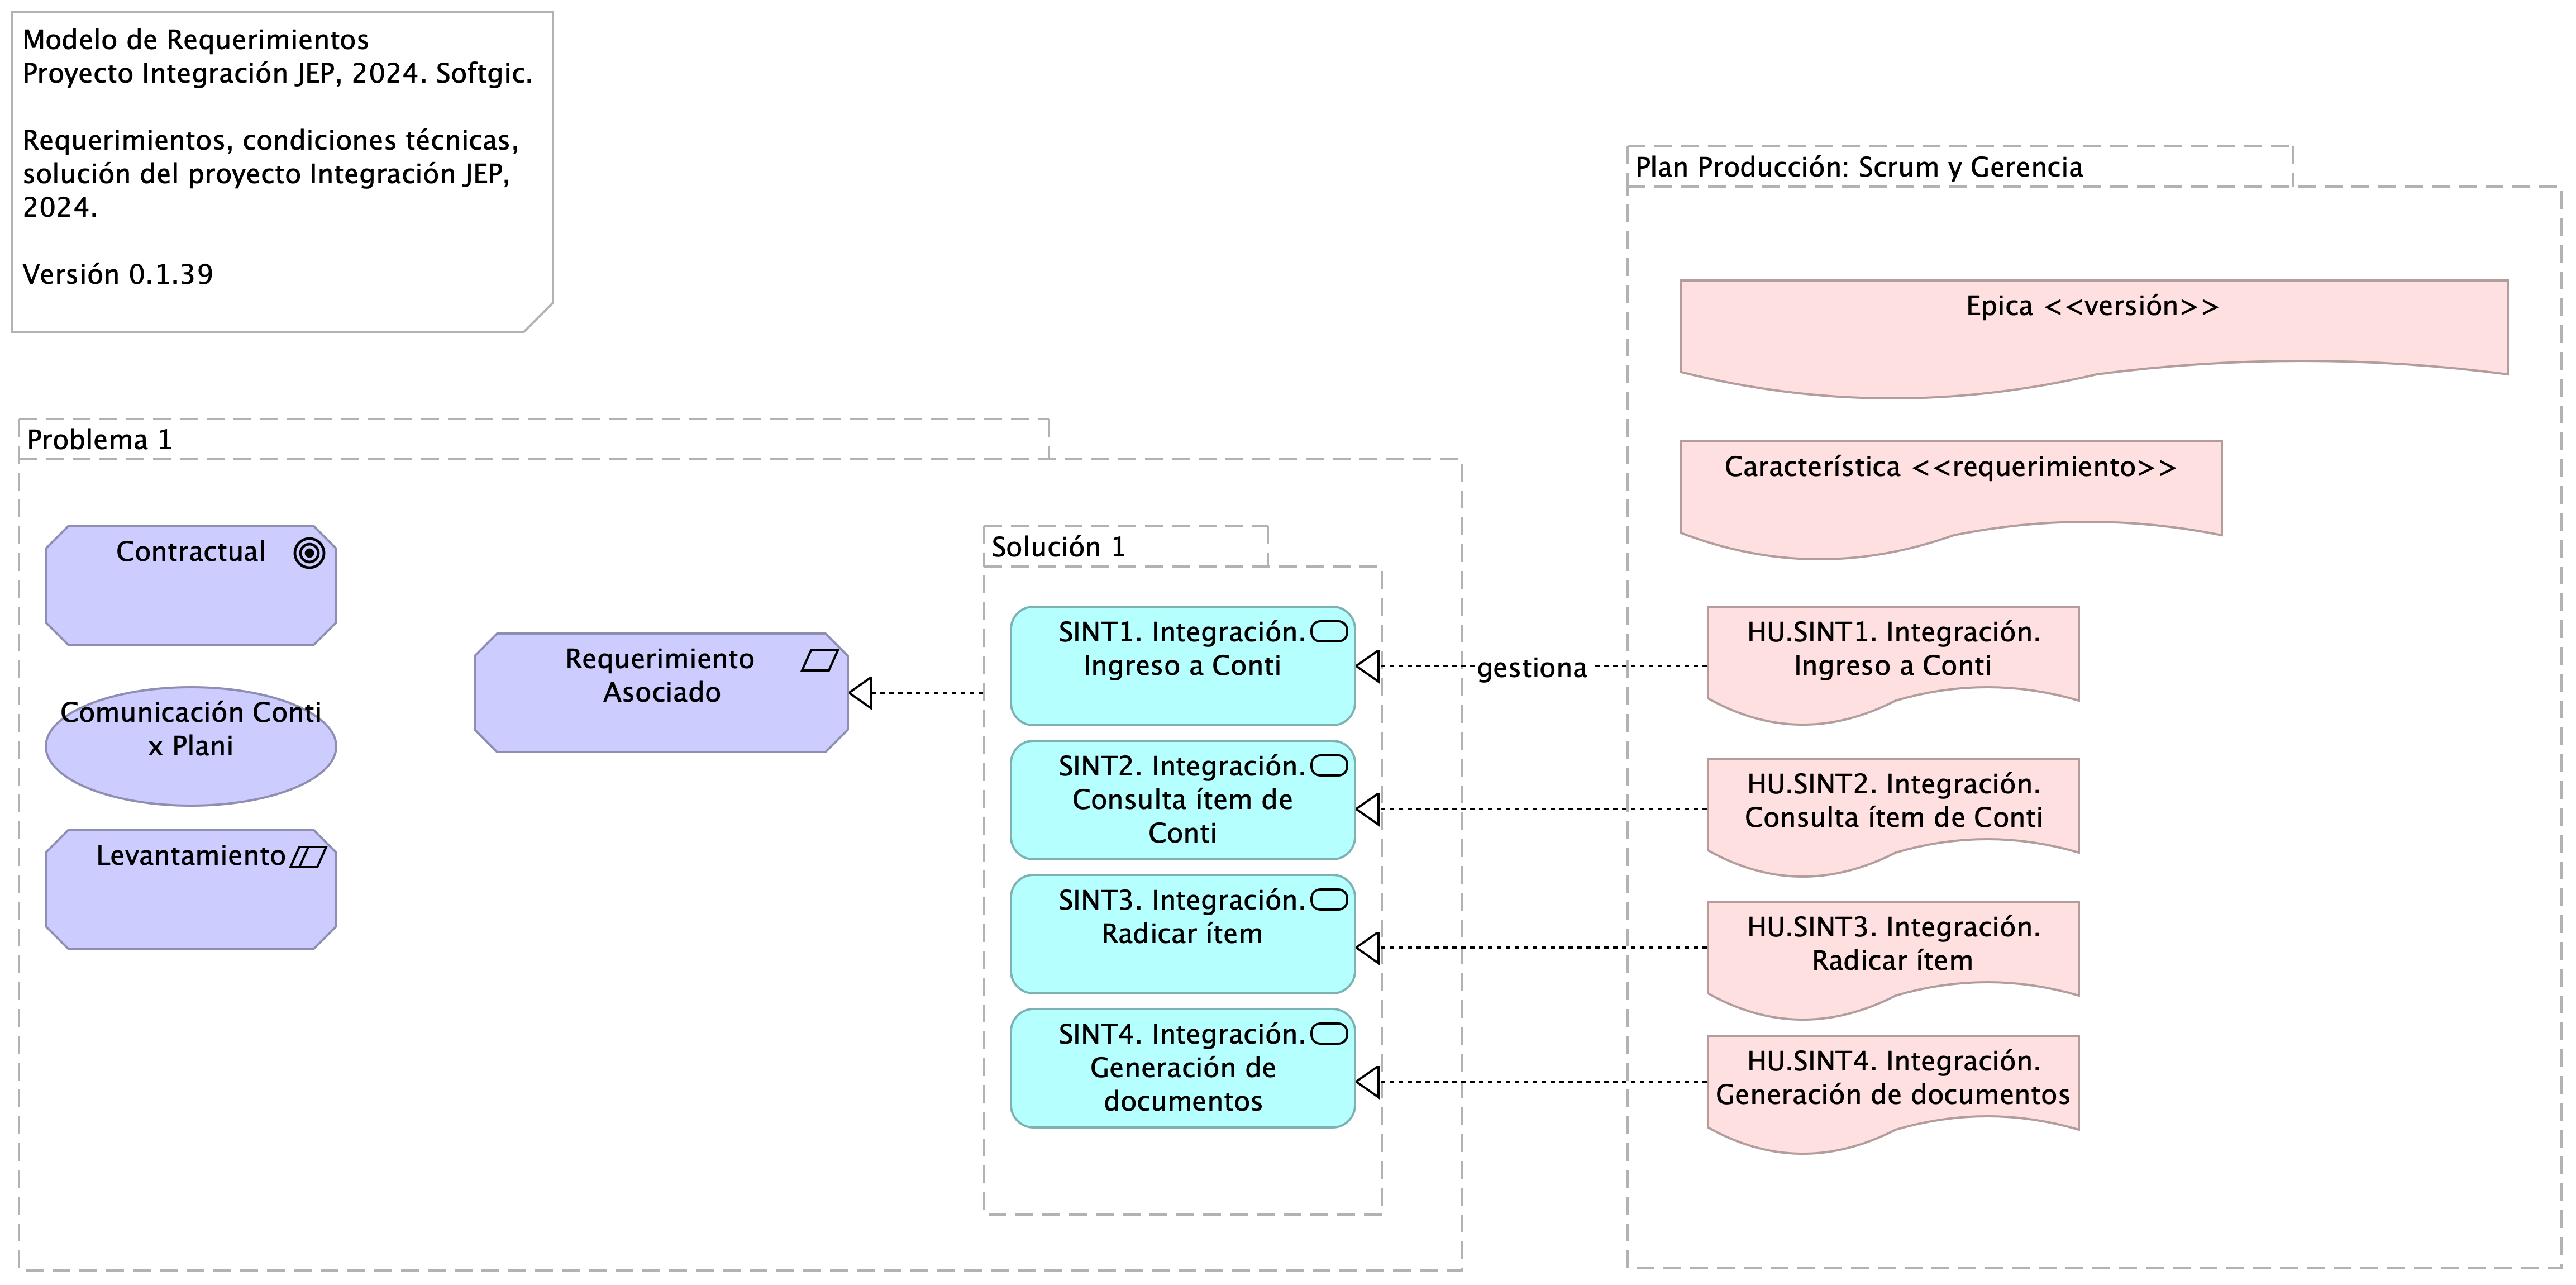
\includegraphics[width=\textwidth,height=5.20833in]{03.1a.contd.vista.png}
\caption{05.REQR.1n.1a. Requerimiento}
\end{figure}

Del alcance del proyecto,

\begin{enumerate}
\def\labelenumi{\arabic{enumi}.}
\tightlist
\item
  Implementación de 20 o más servicios de integración al 31 de diciembre
  del 2024.
\item
  Soporte solución de integración a julio 2025.
\end{enumerate}

Establecemos las bases para el modelo de requerimientos de esta
solución, el cual limita la demanda a:

\begin{itemize}
\tightlist
\item
  Desarrollar únicamente nuevos servicios de integración con el patrón
  de integración empresarial (ESB, Camel K de Apache) propuesto en el
  modelo de interoperabilidad de esta solución.
\item
  Implementar en esta solución de integración las condiciones
  tecnológicas JEP, entendidas como requerimientos no funcionales de
  arquitectura, presentes en el Anexo Nro. 1.1 -- Anexo técnico
  evolución plataforma de interoperabilidad -- Ficha Técnica.
\item
  No son requerimientos de este proyecto el implementar otro tipos de
  requerimientos no expresados aquí, como por ejemplo, migrar los
  servicios existentes de modelo integración directa (EIA) esta solución
  de integración empresarial, o implementar soluciones en las
  aplicaciones de software de la JEP.
\end{itemize}

Para la implementación de los ítems relacionados en el Anexo Nro. 1.1 --
Anexo técnico evolución plataforma de interoperabilidad -- Ficha Técnica
la hoja ``Categorías de Cotización'' contiene las necesidades a
contratar en el ámbito de la evolución tecnológica del modelo de
interoperabilidad y los desarrollos de interoperabilidad tanto con
sistemas internos, como con entidades externas. En la hoja ``Estándares
Desarrollo y Producto'' del archivo mencionado se indican los estándares
recomendados por el fabricante, para tener en cuenta en la entrega de
los servicios que se cotizan.

El Anexo Nro. 1.2 -- Acuerdos de Niveles de Servicio, explica el
procedimiento con el que se dará atención a consultas o solución de
incidencias, tanto en los sistemas operativos, como en los servicios de
interoperabilidad existentes en la actualidad y aquellos que se
contratarán en este proceso, en el sistema Bus de Interoperabilidad
implementado en la Jurisdicción Especial para la Paz.

Fuente: Justificativo de la Contratación Invitación Pública.

\subsection{Problema 1}\label{sec:problema-1}

\subsubsection{Levantamiento}\label{sec:levantamiento}

Restricción: el requerimiento está condicionado por la completitud del
levantamiento.

\subsubsection{Contractual}\label{sec:contractual}

Objetivo: el requerimiento tiene carácter contractual.

\subsubsection{REQR3. Integración con Sistema Conti x
Plani}\label{sec:reqr3.-integraciuxf3n-con-sistema-conti-x-plani}

Atendiendo la necesidad de la Subdirección de Contratación de
implementar el flujo de gestión precontractual en el sistema de Gestión
Documental - Conti se requiere contar con la información de los ítems
del Plan Anual de Adquisiciones -- PAA para iniciar el proceso, la cual
se encuentra gestionada en el Sistema de Gestión y Planeación
Institucional PLANi.

\subsubsection{Índice de la documentación (casos de
uso)}\label{sec:uxedndice-de-la-documentaciuxf3n-casos-de-uso}

\begin{enumerate}
\def\labelenumi{\arabic{enumi}.}
\tightlist
\item
  Integración. Ingreso a Conti
\item
  Integración. Consulta ítem de Conti
\item
  Integración. Radicar ítem 1.Integración. Generación de documentos
\end{enumerate}

\subsubsection{Solución 1}\label{sec:soluciuxf3n-1}

\paragraph{SINT1. Integración. Ingreso a
Conti}\label{sec:sint1.-integraciuxf3n.-ingreso-a-conti}

Tareas de desarrollo

\begin{itemize}
\tightlist
\item
  Interoperabilidad IOP1. Transporte / Entrega Consulta Negocio
\item
  Modelo de datos (XML, RBDMS, \ldots)
\item
  Esquema de datos (XSD, DTD, JSON-E\ldots)
\item
  Contratos de interoperabilidad (WSDL, API\ldots)
\item
  Mensajes petición IN (API, XML\ldots)
\item
  Mensajes respuesta OUT (API, XML\ldots)
\item
  Mensajes excepción (API, XML\ldots)
\item
  Transporte (REST, SOAP)
\item
  Función lógica (JEE, \ldots)
\item
  Registro y envío de actividad
\end{itemize}

\paragraph{SINT2. Integración. Consulta ítem de
Conti}\label{sec:sint2.-integraciuxf3n.-consulta-uxedtem-de-conti}

Tareas de desarrollo

\begin{itemize}
\tightlist
\item
  Interoperabilidad IOP1. Transporte / Entrega Consulta Negocio
\item
  Modelo de datos (XML, RBDMS, \ldots)
\item
  Esquema de datos (XSD, DTD, JSON-E\ldots)
\item
  Contratos de interoperabilidad (WSDL, API\ldots)
\item
  Mensajes petición IN (API, XML\ldots)
\item
  Mensajes respuesta OUT (API, XML\ldots)
\item
  Mensajes excepción (API, XML\ldots)
\item
  Transporte (REST, SOAP)
\item
  Función lógica (JEE, \ldots)
\item
  Registro y envío de actividad
\end{itemize}

\paragraph{SINT3. Integración. Radicar
ítem}\label{sec:sint3.-integraciuxf3n.-radicar-uxedtem}

Tareas de desarrollo

\begin{itemize}
\tightlist
\item
  Interoperabilidad IOP1. Transporte / Entrega Consulta Negocio
\item
  Modelo de datos (XML, RBDMS, \ldots)
\item
  Esquema de datos (XSD, DTD, JSON-E\ldots)
\item
  Contratos de interoperabilidad (WSDL, API\ldots)
\item
  Mensajes petición IN (API, XML\ldots)
\item
  Mensajes respuesta OUT (API, XML\ldots)
\item
  Mensajes excepción (API, XML\ldots)
\item
  Transporte (REST, SOAP)
\item
  Función lógica (JEE, \ldots)
\item
  Registro y envío de actividad
\end{itemize}

\paragraph{SINT4. Integración. Generación de
documentos}\label{sec:sint4.-integraciuxf3n.-generaciuxf3n-de-documentos}

Tareas de desarrollo

\begin{itemize}
\tightlist
\item
  Interoperabilidad IOP1. Transporte / Entrega Consulta Negocio
\item
  Modelo de datos (XML, RBDMS, \ldots)
\item
  Esquema de datos (XSD, DTD, JSON-E\ldots)
\item
  Contratos de interoperabilidad (WSDL, API\ldots)
\item
  Mensajes petición IN (API, XML\ldots)
\item
  Mensajes respuesta OUT (API, XML\ldots)
\item
  Mensajes excepción (API, XML\ldots)
\item
  Transporte (REST, SOAP)
\item
  Función lógica (JEE, \ldots)
\item
  Registro y envío de actividad
\end{itemize}

\subsubsection{Comunicación Conti x
Plani}\label{sec:comunicaciuxf3n-conti-x-plani}

Valor: el requerimientos genera entregables de valor para la integración
de aplicaciones de JEP.

\end{document}
